
\section{Plan}
\label{sec:plan}

Figure~\ref{fig:gantt_chart} displays the project plan as a Gantt
chart. We hope that our initial model needs few adjustments so that we
may spend less time in part 3 and more time comparing experimental
designs (part 4). It is most important to complete 2.1 to test our
hypothesis that growth is not independent. Beyond this goal we would
particularly like to study the effects of randomisation on fitness
estimates (part 4.3) and may bring this forward if we are short on
time. If you would like to follow the project a blog is set up at
http://boo62.github.io/ and useful content will be posted soon.

\end{multicols}
\graphicspath{{images_low_res/}}
\begin{Figure}
  \centering
  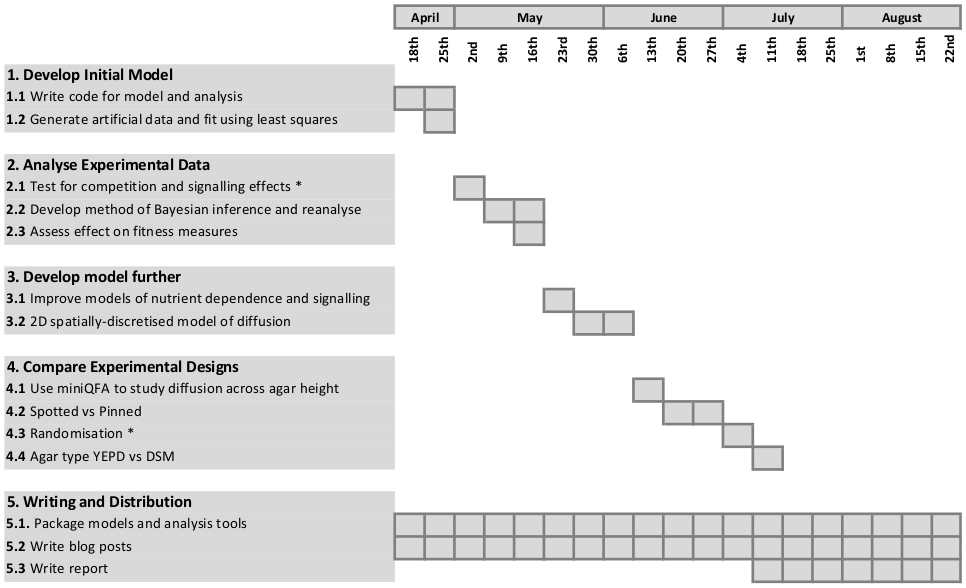
\includegraphics[width=0.98\linewidth]{gantt_chart}
  \captionof{figure}{Gantt chart showing project plan. * marks important events.}
  \label{fig:gantt_chart}
\end{Figure}
\begin{multicols}{2}
% flow chart showing cyclical nature of investigation

%%% Local Variables:
%%% mode: latex
%%% TeX-master: "proposal"
%%% End:
